\newpage

\section{Opracowanie wyników}

Strukturę $\mathbf{Ga_{2}S_{3}}$ można przedstawić w postaci grup $\mathbf{[GaS_{4}]}$. Siarka jest zlokalizowana na wierzchołkach tetraedru, a gal jest zlokalizowany w środku.

\begin{figure}[H]
	\begin{center}
		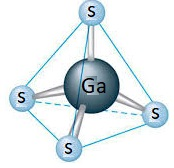
\includegraphics[width=0.3\linewidth]{Opracowanie/tetraedr.jpg}
		\caption{Grupa $\mathbf{Ga_{2}S_{3}}$.}
	\end{center}
\end{figure}

Drania fononów można podzielić na dwie grupy:
\begin{itemize}
	\item Drgania o niskiej energii. Drgania niskoenergetycznych fononów, dla których przesunięcie pików na widmie polaryzacyjnym jest mniejsze od 200 $cm^{-1}$. Do tej grupy należą piki o numerach: 1, 2, 3;
	\item Drgania o wysokiej energii. Drgania wysokoenergetyczne fononów, dla których przesunięcie pików na widmie polaryzacyjnym jest większe od 200 $cm^{-1}$. Do tej grupy należą piki o numerach 4, 5, 6, 7;
\end{itemize}

Częstotliwość drgań można przedstawić za pomocą wzoru:
\begin{equation}
	\omega = \sqrt{\frac{k}{m}}
\end{equation} 

\begin{itemize}
	\item $\omega$ -- częstotliwość drgań;
	\item $k$ -- stałą sprężystości, która zależy od siły oddziaływania między drgającym atomami;
	\item $m$ -- masa atomów.
\end{itemize}

Drgania w ramach jednego tetraedru odpowiada drganiom o wysokiej energii, dla tego że siły wiązania między cząsteczkami w tym samym tetraedrze są duże. Natomiast drgania między cząsteczkami, które się znajdują w różnych tetraedrach są niskoenergetyczne.

Przed rozpoczęciem pomiaru szukaliśmy pod mikroskopem kryształek który przypomina sześciokąt, bo przy pomiarach kryształku w postaci sześciokąta można określić jego osie krystalograficzne.

Chociaż mamy strukturę jednoskośną, przy określonym kierunku kryształ rośnie w postaci sześciokątów. Niżej zostały przedstawione struktury wygenerowane programem VESTA dla struktur $\alpha'$-$Ga_{2}S_{3}$, $\alpha$-$Ga_{2}S_{3}$ i  beta:

\begin{center}
	\begin{figure}[H]
		\begin{minipage}[h]{0.47\linewidth}
			\center{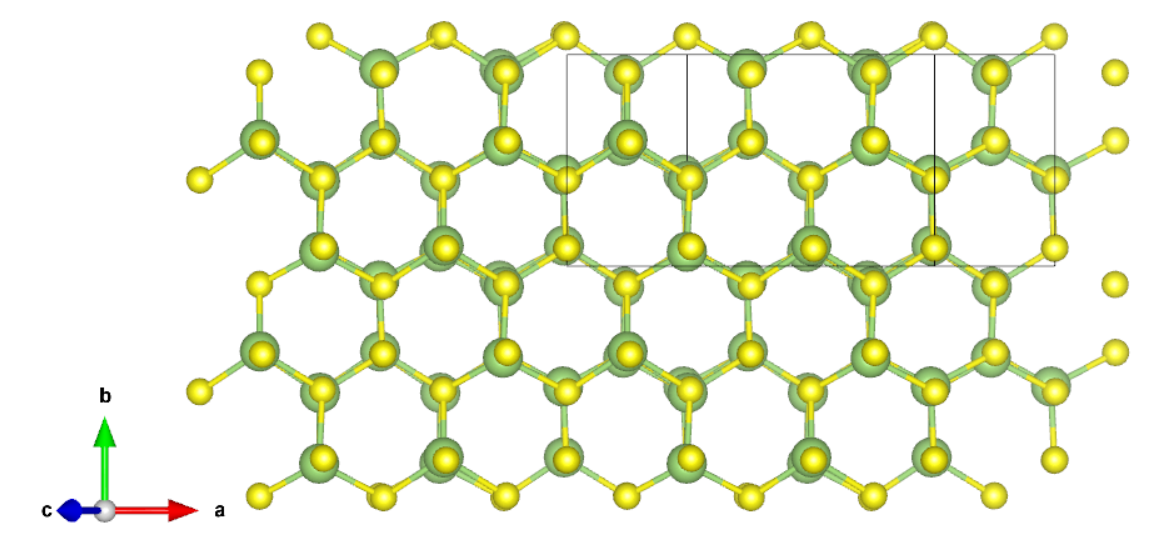
\includegraphics[width=0.8\linewidth]{Opracowanie/alfa_prim_Cc.png}} \\a)
		\end{minipage}
		\hfill
		\begin{minipage}[h]{0.47\linewidth}
			\center{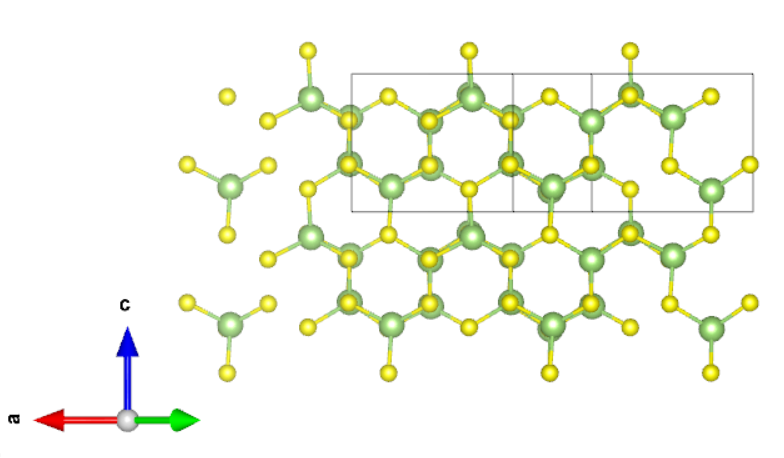
\includegraphics[width=0.8\linewidth]{Opracowanie/alfa_prim_Bb.png}} \\b)
		\end{minipage}
		\caption{a) Struktura krystaliczna $\alpha'$-$\mathbf{Ga_{2}S_{3}}$, grupa przestrzenna Cc. Osie krystalograficzne a i b są prostopadłe i leżą w jednej płaszczyźnie i odpowiadają osiom kartezjańskim x i y. Oś krystalograficzna c jest prostopadła do b i skierowana pod kątem 121$^{\circ}$ do a i skierowana pod kątem 31$^{\circ}$ do osi kartezjańskiej z. b) Struktura krystaliczna $\alpha'$-$\mathbf{Ga_{2}S_{3}}$, grupa przestrzenna Bb. Osie krystalograficzne a i c są prostopadłe i leżą w jednej płaszczyźnie i odpowiadają osiom kartezjańskim x i z. Oś krystalograficzna b jest prostopadła do c i skierowana pod kątem 141$^{\circ}$ do a, i skierowana pod kątem 51$^{\circ}$ do osi kartezjańskiej y. Przygotowano używając oprogramowanie VESTA.[5]}
	\end{figure}
\end{center}

\begin{center}
	\begin{figure}[H]
		\begin{minipage}[h]{0.47\linewidth}
			\center{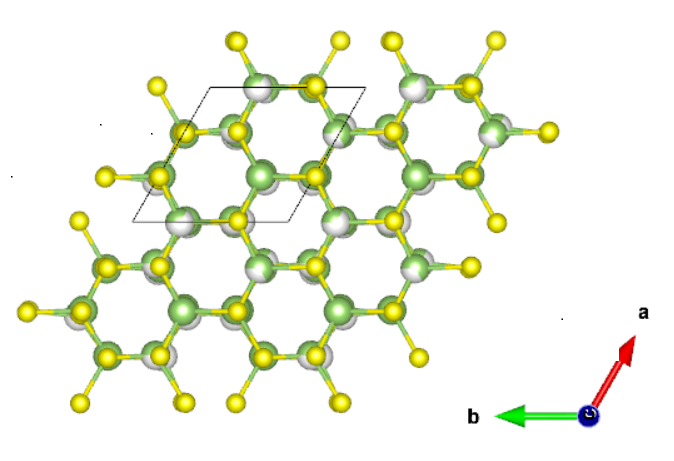
\includegraphics[width=0.8\linewidth]{Opracowanie/alfa.png}} \\a)
		\end{minipage}
		\hfill
		\begin{minipage}[h]{0.47\linewidth}
			\center{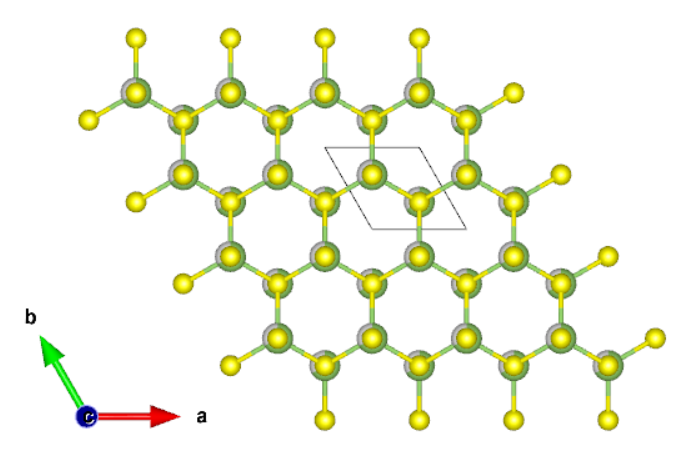
\includegraphics[width=0.8\linewidth]{Opracowanie/beta.png}} \\b)
		\end{minipage}
		\caption{a) Struktura krystaliczna $\alpha$-$\mathbf{Ga_{2}S_{3}}$. Osie krystalograficzne a i b są skierowane pod kątem 120$^{\circ}$ i leżą w jednej płaszczyźnie. Oś krystalograficzna a odpowiada osi kartezjańskiej x, a oś krystalograficzna b jest skierowana pod kątem 30$^{\circ}$ do osi kartezjańskiej y. Oś krystalograficzna c odpowiada osi kartezjańskiej z i jest prostopadła do płaszczyzny w której leżą a i b. b) Struktura krystaliczna $\beta$-$\mathbf{Ga_{2}S_{3}}$. Konfiguracja osi jest taka sama jak w a). Przygotowano używając oprogramowanie VESTA.[5]}
	\end{figure}
\end{center}

Parametrem odpowiedzi modu drgającego na wzbudzenie jest tensor ramanowski, wzór (1). Wektory $e_{i}$ i $e_{s}$ dla naszego układu zależą od jednej z dwóch konfiguracji:
\begin{itemize}
	\item Dla konfiguracji VV wektory mają następującą postać:
	\begin{itemize}
		\item $e_{i} = [\cos \alpha, \sin \alpha, 0]$;
		\item $e_{s} = [\cos \alpha, \sin \alpha, 0]$.
	\end{itemize}
	\item Dla konfiguracji VH wektory mają następującą postać:
	\begin{itemize}
		\item $e_{i} = [\cos \alpha, \sin \alpha, 0]$;
		\item $e_{s} = [-\sin \alpha, \cos \alpha, 0]$.
	\end{itemize}
\end{itemize}

Tensor dla struktury jednoskośnej jest następujący:

\begin{figure}[H]
	\begin{center}
		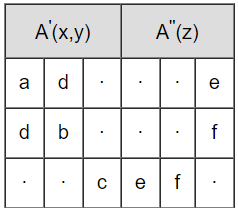
\includegraphics[width=0.3\linewidth]{Opracowanie/Tensor-Cc.png}
		\caption{Tensory ramanowskie dla struktury jednoskośnej.}
	\end{center}
\end{figure}

Dla pików 1, 4, 7 widmo polaryzacyjne dla VH jest przekręcone o kąt 90$^{\circ}$ względem VV. Więc tensor ramanowski dla tych pików przedstawia się jedną macierzą. Ponieważ widmo polaryzacyjne VH nie jest przekręcone o 90$^{\circ}$ dla pozostałych pików, wnioskujemy, że tensor ramanowski dla tych pików jest kombinacją liniową tensorów. 



